\documentclass[11pt]{article}

\usepackage{booktabs}
%\usepackage[margin=0.5in]{geometry}
\usepackage{fullpage}
\usepackage{palatino}
\usepackage{tabularx}
\usepackage{streamit}

\newif\ifprerel
\prereltrue

\newcommand{\new}{\marginpar{\footnotesize \textbf{~~--~New~--}}}
\newcommand{\old}{\marginpar{\footnotesize \textbf{~~--~Old~--}}}

\def\note{\trivlist \small\item\relax\textbf{Note:}}
\def\endnote{\endtrivlist}

% Make picture sizes be sane:
%BEGIN IMAGE
\setlength{\unitlength}{\baselineskip}
%END IMAGE

% Please look the other way, this is a little gross.
\catcode`\$=12
\title{StreamIt Language Specification\\
Version 3.0\ifprerel\thanks{
This document is the latest working version of the language specification.\hfil\break\ttfamily
\hbox{$Id: streamit-lang.tex,v 1.27 2006-04-25 17:55:56 thies Exp $}
}\fi}
\author{\texttt{streamit@cag.csail.mit.edu}}
\catcode`\$=3

\begin{document}

\maketitle
\tableofcontents

\section{Introduction}

StreamIt is a language intended to simplify coding of
signal-processing and other streaming computations.  The programmer
constructs a stream graph, containing blocks with a single input and a
single output, and describes the function of atomic blocks and the
structure of composite blocks.  The compiler generates code for each
block, and applies optimizations to the stream graph to produce
efficient code for the target architecture.

The current implementation of the StreamIt compiler translates the
syntax described in this document to Java code, which can then be
either run against a Java library or compiled to C code and linked
with a runtime library.  Since the compiler can reconstruct the stream
graph, it can combine adjacent filters, or split computationally
intensive filters into multiple parts, or duplicate filters to have
more parallel computation.

The StreamIt language is vaguely reminiscent of other imperative
languages such as C or Java.  In particular, the bodies of filter work
functions and stream initialization code is generally legal Java
code.

\section{Types}

This section describes the various data and object types used in
StreamIt programs.  Data types are passed along tapes between stream
objects, and can be used as local variables.  Stream objects are only
created in initialization code and form a static stream graph.

\subsection{Data Types}

Data types are always created atomically.  They are of fixed size, and
are generally statically allocated.

\subsubsection{Primitive Types}
\label{sec:primitive-types}

The following primitive types exist in StreamIt:

\begin{description}
\item[\lstinline|boolean|]  Either \lstinline|true| or
  \lstinline|false|.

\item[\lstinline|bit|]  A one-bit unsigned integer type, containing
  the value \lstinline|0| or \lstinline|1|.

\item[\lstinline|int|]  A signed integer type, of unspecified length.
  This length will typically be the native word length on the target
  machine; for RAW and x86 compilation, this is usually 32 bits.

\item[\lstinline|float|]  A floating-point type, of the best precision
  that will give good performance.  On x86 this is a double-precision
  float, since computation with single-precision floats is implicitly
  converted to double-precision; on RAW, this is single-precision,
  since that is all that is supported in hardware.

\item[\lstinline|complex|]  A floating-point complex type, of the same
  precision as \lstinline|float|.  This has real and imaginary parts,
  which can be directly accessed with \lstinline|c.real| and
  \lstinline|c.imag|.
\end{description}

\label{sec:operators}
A number of operations are supported on these primitive types; these
are listed in Table \ref{tab:primitive-operators}.  In a binary or
ternary expression, if two expressions are of different primitive
types, they are promoted to the lowest type on the list above.  Real
expressions converted to \lstinline|complex| have an imaginary part of
zero.  \lstinline/|/, \lstinline|&|, and \lstinline|^| are bitwise or,
and, and exclusive-or operators, respectively; \lstinline|!| is a
boolean not.  The boolean logic
operators \lstinline|&&| and \lstinline/||/ behave as in C: they are
short-circuiting, integer values of exactly zero are false, and other
values are true.  \lstinline|==| and other comparison operators return
a boolean value.

\begin{table}
\begin{center}
\begin{tabular}{ccl}
\toprule
\textbf{Operators} & \textbf{Types} \\
\midrule
\lstinline|?:| & Any & First part must be \lstinline|boolean| \\
\lstinline/||/ & \lstinline|int|, \lstinline|bit|, \lstinline|boolean| \\
\lstinline|&&| & \lstinline|int|, \lstinline|bit|, \lstinline|boolean| \\
\lstinline/|/, \lstinline|&|, \lstinline|^| &
  \lstinline|int|, \lstinline|bit| \\
\lstinline|==|, \lstinline|!=| & Any \\
\lstinline|<|, \lstinline|<=|, \lstinline|>|, \lstinline|>=| &
  \lstinline|int|, \lstinline|float| \\
\lstinline|+|, \lstinline|-| &
  \lstinline|int|, \lstinline|float|, \lstinline|complex| \\
\lstinline|*|, \lstinline|/|, \lstinline|%| &
  \lstinline|int|, \lstinline|float|, \lstinline|complex| &
  \lstinline|%| must be \lstinline|int| \\
\lstinline|(cast)| & Any \\
\lstinline|!| & \lstinline|boolean| \\
\lstinline|++|, \lstinline|--| & \lstinline|int| \\
\bottomrule
\end{tabular}
\end{center}
\caption{Operators on primitive types}
\label{tab:primitive-operators}
\end{table}

\subsubsection{Structures}
\label{sec:data-structures}

Named structures of heterogeneous data types are supported.  A
structure must be of a fixed size.  It contains a set of fields, each
of which has a name and a data type.  Any primitive or array type, and
any structure type which has been previously declared in the program,
may be used; recursive structures are not allowed.  The following two
structure definitions are both legal:

\begin{lstlisting}{}
struct A {
  int a;
  int[4] b;
}

struct B {
  A a;
  A[4] b;
}
\end{lstlisting}

A structure definition contains the keyword \lstinline|struct|, the name
of the structure, an open brace, a listing of field (variable)
declarations, and a close brace.  It is not followed by a semicolon.

The only supported operations on structures are field references and
copying.  Field references are of the form \lstinline|a.b|; \lstinline|a| must
be of some structure type \lstinline|A|, and \lstinline|b| must be a field named
in the structure declaration of \lstinline|A|.  The type of this expression
is the declared type of the field.  Note that a similar syntax is used
for referencing the real and imaginary parts of complex numbers; there
is an implicit structure declaration

\begin{lstlisting}{}
struct complex {
  float real, imag;
}
\end{lstlisting}{}

\noindent
along with some syntactic sugar to make complex arithmetic work.

\subsubsection{Arrays}

Arrays of any data type described here are supported.  Arrays must be
of a fixed length.  Array types are written with the base type name,
followed by a single dimension in square brackets.  Multi-dimensional
arrays or matrices are supported as arrays of arrays.

\subsubsection{Variable Declarations}

Variable declarations appear in structure declarations, as well as in
code blocks and stream declarations.  A variable declaration may
declare one or multiple variables, possibly with initializers;
multiple variables are separated with commas.  Of note, the syntax for
array declarations is different from C and Java.  A correct
declaration is \lstinline|int[4] rgbi;|, with the entire type stated
before the variable name.  A static array initializer may be provided
as in C and Java, for example:

\begin{lstlisting}{}
int[3][2] arr = {{1, 2}, {3, 4}, {5, 6}};
\end{lstlisting}{}

If there is no initializer for an array, then all elements are
automatically initialized to a value of zero.

\subsection{Stream Types}

Computation in StreamIt is performed within stream objects.  Every
stream object has an input type and an output data type; the object is
connected to ``tapes'' of a hypothetically infinite number of
homogeneous data objects.  \emph{Filters} are atomic, and have
initialization code and steady-state work code; \emph{pipelines},
\emph{splitjoins}, and \emph{feedback loops} are all composite
structures that include some number of stream objects as children.

All stream objects have initialization code that runs when the object
is first created.  For filters, this code may be omitted, and
generally just sets up filter-local state.  For composite objects, the
initialization code is responsible for creating the child objects.
Filters also have one or more \emph{work functions}, which are called
each time the filter executes.

\paragraph{I/O types.}  Each stream declared at the top level must
also explicitly declare its input and output types.  This is a
declaration like \lstinline|int->int| or \lstinline|float->complex|;
the first type is the stream's input type, the second its output type.
Either type may be \lstinline|void|; in this case, the stream has no
input or output, as appropriate.  If it is a filter, it must not
declare a peek, pop, or push rate.  The top-level stream in a
program has type \lstinline|void->void|; no other streams of this type
are allowed.

\subsubsection{Stream Parameters}

A stream may have a set of parameters provided to it.  These
parameters are available to all functions within the stream type, and
may not be changed.  Values for these parameters must be passed in
when the stream is created.  Stream parameters are declared with types
and names in a parenthesized list after the name of the stream; when a
stream it instantiated, values for the parameters must follow the name
of the stream.  For example:

\begin{lstlisting}{}
// declaration
float->float filter MatrixMatrixMultiply(int A,
                 int B, int C) { ... }

void->void pipeline Toplevel() {
  add Source();
  // instantiation
  add MatrixMatrixMultiply(3, 5, 4);
  add Sink();
}
\end{lstlisting}

Note that it is also possible to pass a parameterized-length array as
a parameter to a stream, so long as the length is also passed as a
parameter. For example, the following is a legal filter declaration:

\begin{lstlisting}{}
int->int filter FIR (int N, int[N] weights) { ... }
\end{lstlisting}

\paragraph{Compile-time constants.}  Several things in StreamIt must
be \emph{compile-time constant}; for example, the I/O rates of a
filter must be determined at {\old} compile-time, and the compiler must be
able to statically create the expanded stream graph.  An expression is a
compile-time constant if it is a literal, a stream parameter, or an
expression whose components are compile-time constants.

\subsubsection{Parameterized Stream Types}

Stream types may be \emph{parameterized} on some data type or types,
much like ``template'' types in C++.  This may be used for
data-reordering operations, and is used for several cases of built-in
filters.

Parameterized objects cannot currently be created by the user.  To
instantiate a built-in parameterized type, use the name of the stream
type, followed by the name of the data type in angle brackets, such as
\lstinline|Identity<int>|.

\begin{note}
User-instantiated parameterized types are a future StreamIt
extension.
\end{note}

\subsubsection{Filters}

All computation in StreamIt takes place within filters.  Filters must
explicitly declare their initialization code if present, but also have
the option of omitting it.  A filter has a single {\old} work function.
%; it may also declare other phase functions.  Each
The work
%or phase 
function must declare its \emph{I/O rates}, the number of items 
%one call to the function 
it removes, examines, or places on its tape.  A basic filter
declaration looks like this:

\begin{lstlisting}{}
int->int filter IntAvgFilter {
  init {
    // empty
  }
  work pop 1 peek 2 push 1 {
    push(peek(0) + peek(1));
    pop();
  }
}
\end{lstlisting}

This filter is named \lstinline|IntAvgFilter|; it reads integers off of its
input tape, and writes integers to its output tape.  Each execution of
the work function removes exactly one item from the input tape and
examines at most two items; it causes exactly one item to be pushed on
to the output tape.

%% Commenting out because of keep.
%%
%% All computation in StreamIt takes place within filters.  Filters must
%% explicitly declare their initialization code if present, but also have
%% the option of omitting it.  A filter has a single work function; it
%% may also declare other phase functions.  Each work or phase function
%% must declare its \emph{I/O rates}, the number of items one call to the
%% function removes, examines, or places on its tape.  A basic filter
%% declaration looks like this:

%% \begin{lstlisting}{}
%% int->int filter IntAvgFilter {
%%   init {
%%     // empty
%%   }
%%   work pop 1 peek 2 push 1 keep 1 {
%%     push(keep(0) + peek(1));
%%     pop();
%%   }
%% }
%% \end{lstlisting}

%% This filter is named \lstinline|IntAvgFilter|; it reads integers off
%% of its input tape, and writes integers to its output tape.  Each
%% execution of the work function removes exactly one item from the input
%% tape and examines at most two items; it causes exactly one item to be
%% pushed onto the output tape, and looks at the item pushed on the
%% previous iteration.

\paragraph{Init functions.}  Init functions are declared using the
keyword \lstinline|init|.  They take no parameters.  They may initialize
filter fields or do other work, but have no access to the filter's
tapes.

\paragraph{Filter state.}  The top level of the filter may include
variable declarations.  These variables are visible to every function
in the filter, and may be used to carry state between iterations of
the work function.  We refer to these variables as {\it fields} of the
filter.  For example, the variable \lstinline|i| is a field of the
following filter:
\begin{lstlisting}{}
void->int filter Counter {
  int i = 0;
  work push 1 {
    push(i++);
  }
}
\end{lstlisting}{}

\paragraph{Work functions.}  Work functions are declared using the
keyword \lstinline|work|.  This keyword may be followed by rate
declarations; if these are absent, the filter is a {\old} \emph{phased
filter} (see Section~\ref{sec:phased-filter}).

Rate declarations consist of \lstinline|push rate-expr|,
\lstinline|peek rate-expr|, and \lstinline|pop rate-expr|,
%, and \lstinline|keep expr|, 
in any order.  The push and pop rates specify the number of items
produced and consumed by a given execution of the work function.  The
peek rate specifies the maximum index that is peeked in a given
execution; that is, given a peek rate of $r$, the filter can execute
\lstinline|peek(i)| for all $i < r$.

Each {\new} rate expression is of the form \lstinline|[min, avg, max]|, 
where \lstinline|min| denotes the minimum number of items,
\lstinline|avg| denotes the average number of items (over all
executions), and \lstinline|max| denotes the maximum number of items.
The average rate may optionally be ommitted, in which case the rate
declaration is of the form \lstinline|[min, max]|.  If only one
expression appears, then it represents both the minimum and maximum
rate (i.e., the rates are equal); in this case, the brackets are
ommitted.  For example, a work function that pops exactly 1 item and
pushes between 2 and 4 items, with an average of 3 items, is declared
as follows:

\begin{lstlisting}{}
work pop 1 push [2, 3, 4] { ... }
\end{lstlisting}

The declaration above signifies a {\it dynamic rate} in that the exact
number of items produced on any given execution is unknown at compile
time.  Rate declarations support three forms of dynamism:
\begin{itemize}

\item A rate that falls within a static range, as specified above.

\item A rate that changes intermittently throughout the program.  In
this case, the rate should be declared in terms of a filter field that
is updated occaisionally (for instance, from \lstinline|work| or a
message handler).  For example:

\begin{lstlisting}{}
float->float filter AdaptiveAverage(int initial_N) {
  int N;
  init {
    N = initial_N;
  }
  work push 1 pop 1 peek N {
    // push average of N inputs
    float sum = 0;
    for (int i=0; i<N; i++) {
      sum += peek(i);
    }
    push(sum/((float)N));

    // calculate noise, increase N if necessary
    boolean tooMuchNoise = ... ;
    if (tooMuchNoise) {
      N = N*2;
    }
  }
}
\end{lstlisting}

In the above filter, the peek rate for a given instance of
\lstinline|work| is the value of \lstinline|N| as defined when
\lstinline|work| starts to execute.  Changes made to \lstinline|N|
from within \lstinline|work| effect the rate declaration of the next
execution, but not the current one.

\item A rate that is completely unpredictable.  In this case, the
special token \lstinline|*| may be substituted for one or more of the
\lstinline|min|, \lstinline|avg|, and \lstinline|max| fields in the
declaration.  For example, the following filter pushes one item and
pops an unbounded number of items:

\begin{lstlisting}{}
int->int filter FilterLessThan(int N) {
  work push 1 pop [1,*] {
    while (peek(0) < N) {
      pop();
    }
    push(peek(0));
    pop();
  }
}
\end{lstlisting}

While the \lstinline|*| token allows one to declare filters with
unbounded I/O rates, a concrete upper bound should be provided
whenever possible.  Unbounded I/O rates can drastically degrade
performance, as it becomes difficult (or impossible) to predict the
amount of data needed for a filter to complete an atomic execution.

\end{itemize}

\noindent There is also some syntactic sugar for rate declarations:

\begin{itemize}

\item If the push or pop rate is ommitted, it is assumed to be zero.
The corresponding input or output tape type must be \lstinline|void|.

\item If the peek rate is ommitted, it is assumed to be equal to the
pop rate.

\item If there are no \lstinline|pop| calls at all in the function
body (all access to the input tape is by peeking), the number of items
declared as the pop rate will be automatically popped at the end of
the work function.

\end{itemize}

\paragraph{Prework Functions.}  A filter may specify an additional work 
function that is run in place of the normal work function the first
time the filter executes.  This function uses the \lstinline|prework|
keyword, and is otherwise identical to the normal work function.

Prework functions can be very useful for setting up initial conditions
based on the first set of inputs, or for pushing extra items on the
first invocation.  For example, consider the following implementation
of a Delay:

\begin{lstlisting}{}
float->float filter Delay(int N) {
  prework push N {
    for (int i=0; i<N; i++) {
      push(0);
    }
  }

  work push 1 pop 1{
    push(pop());
  }
}
\end{lstlisting}

\paragraph{Helper functions.}  A helper function performs some
auxiliary bit of computation, and may be called from the init function
or the work function.  A helper function has a list of zero or more
parameters, and returns zero or one values.  A helper function
declaration contains the return type, the name of the function, the
parameter list, and the function body, just like a normal C or Java
function.

\paragraph{Message-handler functions.}  A message handler function
changes the state of the filter in response to some external event,
delivered via a message.  It is declared with the keyword
\lstinline|handler|, the name of the message, the parameter list, and
the function body.  A message handler cannot return a value, so no
return type is declared.

\paragraph{Naming I/O tapes.}  For {\new} documentation 
purposes, a filter's input and output tapes can be given a name as
part of their type declaration.  This name is subsequently used as a
prefix for all push and pop operations.  For example:
\begin{lstlisting}{}
int fullData -> int maskedData filter DoMask {
  work push 1 pop 1 {
    maskedData.push(fullData.pop() & 128);
  }
}
\end{lstlisting}

\subsubsection{Phased Filters}  
\label{sec:phased-filter}

If the work function does not have rate declarations {\old}, it may not
perform \lstinline|push| and \lstinline|pop| operations directly.
However, in a phased filter, it may call \emph{phase functions}, which
are declared like work functions but begin with the keyword
\lstinline|phase| and a name, and always have rate declarations.  The
runtime system ensures that, when a phase function is called, its
\lstinline|peek| and \lstinline|pop| rates are satisfiable, even if
other filters need to run for later phases to execute.  Beyond this
special use, phase functions may not be directly called.  For example:

\begin{lstlisting}{}
int->int filter BlockReader {
  // Each block has a 4-int header, 24 ints of data,
  // and a 4-int footer.
  work {
    readHeader();
    for (int i = 0; i < 24; i++)
      echoData();
    readFooter();
  }
  phase readHeader pop 4
     { pop(); pop(); pop(); pop(); }
  phase echoData pop 1 push 1 { push(pop()); }
  phase readFooter pop 4
     { pop(); pop(); pop(); pop(); }
}
\end{lstlisting}

\subsubsection{Pipelines}

The simplest composite stream is a pipeline.  A pipeline contains a
number of child streams; the output of the first stream is connected
to the input of the second, whose output is connected to the input of
the third, and so on.  A pipeline declaration looks like

\begin{lstlisting}{}
float->complex pipeline FloatToComplexAdd {
  add ReImToComplex();
  add ComplexPairAdd();
}
\end{lstlisting}

The body of the pipeline declaration is the initialization code; no
internal function declarations 
%or message handlers 
are allowed.  In addition to the internal typing constraints mentioned
previously, the input type of the pipeline must match the input type
of the first filter, and the output type of the pipeline must match
the output type of the last filter.

\begin{figure}[htbp]
  \begin{center}
    \begin{picture}(18,9)
      \put(3,9){\vector(0,-1){1}}
      \put(0,1){\framebox(6,7)[lt]{\lstinline|Pipeline|}}
      \put(7,8){\makebox(9,1)[l]{\lstinline|float->float|}}
      \put(7,7){\makebox(9,1)[l]{\lstinline|pipeline Pipeline \{|}}
      \put(3,8){\vector(0,-1){1}}
      \put(1,6){\framebox(4,1){\lstinline|Child1|}}
      \put(7,6){\makebox(9,1)[l]{\lstinline|\ add Child1();|}}
      \put(3,6){\vector(0,-1){1}}
      \put(1,4){\framebox(4,1){\lstinline|Child2|}}
      \put(7,4){\makebox(9,1)[l]{\lstinline|\ add Child2();|}}
      \put(3,4){\vector(0,-1){1}}
      \put(1,2){\makebox(4,1){$\cdots$}}
      \put(7,2){\makebox(9,1)[l]{\lstinline|\ ...|}}
      \put(3,2){\vector(0,-1){1}}
      \put(7,1){\makebox(9,1)[l]{\lstinline|\}|}}
      \put(3,1){\vector(0,-1){1}}
    \end{picture}
    \caption{Pipelines}
    \label{fig:pipeline}
  \end{center}
\end{figure}


\subsubsection{Splitjoins}

A splitjoin allows computation to be run in parallel, possibly using
different parts of the input stream.  It is so named because incoming
data passes through a \emph{splitter}, is redistributed to the child
streams for processing, and then is fed through a \emph{joiner} to be
recombined into a single output stream; see section
\ref{sec:splitters-joiners}.

\begin{lstlisting}{}
int->int splitjoin AddAndSub {
  split duplicate;
  add IntAdder();
  add IntSubtractor();
  join roundrobin;
}
\end{lstlisting}

This splitjoin has two children.  Incoming data is duplicated onto
both streams.  The first branch consumes two elements and adds them;
the second consumes two elements and subtracts them.  The resulting
values are then pushed onto the output stream in a round-robin
fashion, with values from alternating streams.

\begin{figure}[htbp]
  \begin{center}
    \begin{picture}(29,5)
      \put(6,5){\vector(0,-1){1}}
      \put(0,1){\framebox(12,3)[tl]{\lstinline|SplitJoin|}}
      \put(13,4){\makebox(16,1)[l]
        {\lstinline|int->int splitjoin SplitJoin \{|}}
      \put(6,4){\vector(-3,-1){3}}
      \put(6,4){\vector(0,-1){1}}
      \put(6,4){\vector(3,-1){3}}
      \put(13,3){\makebox(16,1)[l]{\lstinline|\ split roundrobin(2);|}}
      \put(1,2){\framebox(4,1){\lstinline|Child1|}}
      \put(5,2){\makebox(2,1){$\cdots$}}
      \put(7,2){\framebox(4,1){\lstinline|ChildN|}}
      \put(13,2){\makebox(16,1)[l]
        {\lstinline|\ add Child1(); ... add ChildN();|}}
      \put(3,2){\vector(3,-1){3}}
      \put(6,2){\vector(0,-1){1}}
      \put(9,2){\vector(-3,-1){3}}
      \put(13,1){\makebox(16,1)[l]{\lstinline|\ join roundrobin;|}}
      \put(6,1){\vector(0,-1){1}}
      \put(13,0){\makebox(16,1)[l]{\lstinline|\}|}}
    \end{picture}
    \caption{Splitjoins}
    \label{fig:splitjoin}
  \end{center}
\end{figure}

\subsubsection{Feedback Loops}

A feedback loop has a body stream.  Its output passes through a
splitter; one branch of the splitter leaves the loop, and the other
goes to the loop stream.  The output of the loop stream and the loop
input then go through a joiner to the body's input.

\begin{lstlisting}{}
float->float feedbackloop AddFeedback(float scaling) {
  join roundrobin;
  body FloatAdder();
  loop FloatScaler(scaling);
  split duplicate;
  enqueue 0.0;
}
\end{lstlisting}

The \lstinline|body| and \lstinline|loop| declarations may be omitted;
if so, an implicit \lstinline|Identity| filter of the appropriate type
is inserted.

\paragraph{Semantics of splitters and joiners.}  Splitters and joiners
both treat the stream input as the first child, and the loop edge as
the second child.  Splitters and joiners that do not allow exactly two
children are disallowed.

\paragraph{\lstinline|enqueue| statement.}  The \lstinline|enqueue|
statement takes a value and places it in FIFO order on the output tape
from the loop stream.  You will generally need to enqueue enough items
that the input joiner will be able to fire once; enqueuing more items
causes a delay in the feedback loop.

\begin{figure}[htbp]
  \begin{center}
    \begin{picture}(21,9)
      \put(3,9){\vector(0,-1){1}}
      \put(10,8){\makebox(11,1)[l]{\lstinline|float->float|}}
      \put(0,1){\framebox(9,7)[lt]{\lstinline|Feedback|}}
      \put(10,7){\makebox(11,1)[l]{\lstinline|feedbackloop Feedback \{|}}
      \put(3,8){\vector(0,-1){1}}
      \put(10,6){\makebox(11,1)[l]{\lstinline|\ join roundrobin;|}}
      \put(3,7){\vector(0,-1){1}}
      \put(1,5){\framebox(4,1){\lstinline|Body|}}
      \put(10,5){\makebox(11,1)[l]{\lstinline|\ body Body();|}}
      \put(3,5){\vector(0,-1){3}}
      \put(3,2){\line(1,0){3}}
      \put(6,2){\vector(0,1){1}}
      \put(4,3){\framebox(4,1){\lstinline|Loop|}}
      \put(10,3){\makebox(11,1)[l]{\lstinline|\ loop Loop();|}}
      \put(6,4){\line(0,1){3}}
      \put(6,7){\vector(-1,0){3}}
      \put(10,2){\makebox(11,1)[l]{\lstinline|\ split roundrobin(4,1);|}}
      \put(3,2){\vector(0,-1){1}}
      \put(10,1){\makebox(11,1)[l]{\lstinline|\ enqueue(0.0);|}}
      \put(3,1){\vector(0,-1){1}}
      \put(10,0){\makebox(11,1)[l]{\lstinline|\}|}}
    \end{picture}
    \caption{Feedback Loop}
    \label{fig:feedback-loop}
  \end{center}
\end{figure}

\subsubsection{Splitters and Joiners}
\label{sec:splitters-joiners}

Splitters have a single input tape and multiple output tapes; joiners
have multiple input tapes and a single output tape.  They appear in
feedback loops and splitjoins.

Splitters {\new} and joiners are programmable, just like filters.  The
only difference is that they declare multiple input or output tapes,
with corresponding mechanisms for declaring I/O rates and accessing
items on the tapes.  There is also a set of predefined splitters and
joiners with special semantics; some of their behaviors cannot be
fully emulated by programmable splitters and joiners.

For example, the following joiner inputs a data value and a boolean
flag; if the flag is true, the data is forwarded to the output.
Otherwise, the data is simply consumed.
\begin{lstlisting}{}
int val, boolean flag -> int joiner Router() {
  work pop 1,1 push [0,1] {
    if (flag.pop()) {
      push(val.pop());
    } else {
      val.pop();
    }
  }
}
\end{lstlisting}

The syntax for filters is extended in the following ways to support
multiple input and output tapes:
\begin{enumerate}

\item The stream is declared using the keyword ``splitter'' or
``joiner'' instead of ``filter''.

\item To declare a fixed number of inputs (resp. outputs), each input
(resp. output) stream must be named, as described for filters.  Each
tape declaration consists of a type and a name; declarations are
separated by commas.  For example:
\begin{lstlisting}{}
complex MyInput1, float MyInput2 -> float MyOutput joiner Foo { ... }
\end{lstlisting}
As in filters, push and pop operations to a named stream follow the
form \lstinline|MyInput1.pop()|.

\item Work functions are annotated with a comma-delineated list of I/O
rates, one for each tape declared by the splitter or joiner.  For
example, a work function that pops one item from its first input, pops
two items from its second input, and pushes 3 items to its output is
declared as follows:
\begin{lstlisting}{}
work pop 1,2 push 3 { ... }
\end{lstlisting}

\item The number of inputs and outputs can also be parameterized.
This is done using array syntax on the {\it name} of the input tape.
For example, a joiner with $N$ integer inputs can be declared:
\begin{lstlisting}{}
int A[N] -> int joiner Bar { ... }
\end{lstlisting}
In this case, pop expressions take the form of \lstinline|A[i].pop()|.
The rate declaration can also be parameterized to indicate a distinct
rate on each input stream.  This is done by preceding the rate
declaration with the quantifier \lstinline|A[i]:|, where $A$ is the
name of the input stream, and $i$ is a free variable that can be used
to specify the rate on the $i$th stream.  For example, the following
joiner performs a ``triangular join'' by reading $i$ items from the
$i$th input stream:
\begin{lstlisting}{}
int A[N] -> int joiner Triangular(int N) {
  work pop A[i]:i push N*(N+1)/2 {
    for (int i=0; i<N; i++) {
      for (int j=0; j<=i; j++) {
	push(A[i].pop());
      }      
    }
  }
}
\end{lstlisting}

If each stream can be described by the same rate declaration, then no
quantification is necessary, and the declared rate applies
independently to each stream.  For example, the following splitter
duplicates each item from the input tape onto each of $N$ output
tapes:
\begin{lstlisting}{}
int A -> int B[N] splitter MyDuplicate(int N) {
  work pop 1 push 1 {
    int val = A.pop();
    for (int i=0; i<N; i++) {
      B[i].push(val);
    }
  }
}
\end{lstlisting}
If there is a dynamic rate declaration for an array of streams, then
each stream might process a different number of items on a given
execution.

As a final example of parameterization, consider a joiner that inputs
integers from $N$ different streams and packs them into an $N$-element
array that is output as a single item:
\begin{lstlisting}{}
int A[N] -> int[N] B joiner Pack(int N) {
  work pop 1 push 1 {
    int[N] result;
    for (int i=0; i<N; i++) {
      result[i] = A[i].pop();
    }
    B.push(result);
  }
}
\end{lstlisting}

\end{enumerate}

The rest of this section describes predefined splitters and joiners
that have special semantics.

\paragraph{\lstinline|duplicate| Splitters.} \lstinline|duplicate| 
splitters take each incoming item and push the same item to each of
the outgoing tapes, duplicating data.  As illustrated previously, the
\lstinline|duplicate| splitter can be implemented within the StreamIt
language.

\paragraph{\lstinline|roundrobin| Splitters and Joiners.}  \lstinline|roundrobin| 
splitters take each item and send it to exactly one of the child
streams, in order.  Either \lstinline|roundrobin| or
\lstinline|roundrobin()| causes one item to be sent to each output, in
order; \lstinline|roundrobin(2)| causes two items to be sent to the
first stream, two to the second, and so on.  \lstinline|roundrobin(2, 4, 2)| 
requires there to be exactly three children, and sends two to
the first child, four to the second, and two to the third.  A
round-robin weight may be 0; in this case, the child input must be of
type \lstinline|void|.  A \lstinline|roundrobin(0)| splitter on a
splitjoin means that no children take any input, and the input type
of the entire splitjoin is \lstinline|void|.

\lstinline|roundrobin| joiners are identical to \lstinline|roundrobin|
splitters, except that they read from the input tapes in the specified
pattern and write data to the output tape.  The \lstinline|roundrobin|
splitters and joiners can also be implemented within the StreamIt
language.

\paragraph{\lstinline|ratio| Splitters and Joiners.}  \lstinline|ratio| 
{\new} splitters and joiners are declared with the same syntax as
round-robin.  However, within a given execution, items may be sent out
of order.  For example, a \lstinline|ratio(2, 3)| splitter processes a
total of 5 items in a single execution; any 2 of the items will go to
the first stream, and the other 3 items will go to the second stream.
One can increase the granularity at which the ratio is maintained by
scaling up all rates by a constant factor.  Note that one or more of
the rates may be dynamic, as indicated by the token \lstinline|*|.  In
particular, a \lstinline|ratio(*, *)| joiner indicates that the
compiler is free to merge items in any pattern.

\paragraph{\lstinline|inorder| Joiners.}  \lstinline|inorder| {\new} 
joiners merge items in the same order that they were produced by the
corresponding splitter.  If there is a change of data rate on a given
path of a splitjoin, then items are merged according to the stream
dependence relation as used by the messaging system.

\subsubsection{Anonymous Streams}
\label{sec:anonymous-streams}

It is possible to declare a stream object without a name, if it is
used in exactly one place in the program.  In general anonymous stream
declarations look exactly like the corresponding normal stream
declaration, except that the stream type is optional for non-filter
streams and the name is omitted.  The semicolon that normally ends the
\lstinline|add|, \lstinline|body|, or \lstinline|loop| statement is
optional in this case.

\begin{lstlisting}{}
complex->float feedbackloop FeedbackMagnitude(float scaling) {
  join roundrobin;
  body complex->float filter {
    work pop 2 push 1 {
      push(abs(peek(0) * peek(1)));
      pop(); pop();
    }
  };
  loop pipeline {
    add float->float filter {
      work pop 1 push 1 { push(pop() * scaling); }
    };
    add FloatToComplex();
  };
  split duplicate;
}
\end{lstlisting}

The input and output types of anonymous streams are determined by the
compiler, if these types are not explicitly specified in the code.

Anonymous streams do not have stream parameters.  In certain cases,
though, code within anonymous streams can access variables and stream
parameters from the containing stream.  Values so referenced must be
compile-time constant.  Fields of the containing stream cannot be
accessed, and local variables and stream parameters in the containing
code cannot be modified.

\subsection{Execution Model}

StreamIt does not explicitly assume sequential or parallel hardware.
A component of the stream graph may \emph{fire}, possibly in parallel
with other firings, if its conditions to execute are met.  The
scheduler in the compiler chooses an order to execute filters such
that the firing conditions are met.  A particular back-end may place
additional restrictions on firings; a uniprocessor back-end may
require that only one stream object executes at a time, or a parallel
back-end might add the constraint that two objects may not both be
executing if the output of one is an input of another.  These
constraints are transparent to the programmer, however.

\begin{itemize}
\item A filter may fire when its input has at least as many items as
  its peek rate.
%, and if firing would not leave fewer items on its
%  input than its predecessor's keep rate.  
  It pops its pop rate from the input, and pushes its push rate onto
  its output.
%% \item If a filter has never fired, and it has a prework function, then
%%   the prework function is executed in place of the work function, and
%%   the I/O rates on the prework function are considered when deciding
%%   if the filter may fire.  The prework function is called exactly once.
%% \item A phased filter has a current phase.  Phases are executed in
%%   order according to the static control flow in the work function.
%%   Code between phase invocations may be executed any time between the
%%   preceding and succeeding phases.  The current phase may execute
%%   under the same conditions listed above for a filter; execution of
%%   the phased filter then may pause until the next phase may fire.
\item A joiner in a feedback loop or splitjoin may fire when the
  specified number of items are available on each of its inputs.  It
  pushes the sum of the input weights onto its output.
\item A round-robin splitter may fire when the sum {\old} of the
  number of output items is available on its input, and produces the
  specified number of items on each output.
\item A duplicate splitter may fire when at least one item is
  available on its input.  It pops one item from its input and pushes
  one item to each output.
\end{itemize}

\section{Statements}

This section describes statements legal in StreamIt code.  For the
most part, these are identical to legal statements in C or Java.  Some
statements, particularly those that set up the stream graph, are only
legal in initialization code; other statements are legal anywhere.

\subsection{Initialization-Only Statements}

\subsubsection{\lstinline|add| Statement}

The \lstinline|add| statement adds a child stream to the current stream
object.  It is valid in splitjoins and pipelines only.  In a
splitjoin, it adds a new stream to the end of the current list of
children.  In a pipeline, it adds a new stream to the end of the chain
of children.

This statement takes a \emph{stream constructor}; see section
\ref{sec:expr-stream-constructor}.

\subsubsection{\lstinline|body| Statement}

The \lstinline|body| statement adds a child stream as the body part of
a feedback loop.  This statement must be executed at most once in the
initialization code of a feedback loop, and is invalid anywhere else.
If a feedback loop does not contain a \lstinline|body| statement, an
\lstinline|Identity| filter of the appropriate type is used by
default.

This statement takes a \emph{stream constructor}; see section
\ref{sec:expr-stream-constructor}.

\subsubsection{\lstinline|enqueue| Statement}

The \lstinline|enqueue| statement is valid only within the
initialization code of a feedback loop.  It causes the specified item
to be placed after all other previously enqueued items on the input to
the feedback loop joiner.  This statement takes a single value
expression.

\subsubsection{\lstinline|join| Statement}

The \lstinline|join| statement declares the joiner type of a feedback
loop or splitjoin.  It only appears in initialization code, and is
invalid in initialization code for any other construct.  

\subsubsection{\lstinline|loop| Statement}

The \lstinline|loop| statement adds a child stream as the loop part of
a feedback loop.  This statement must be executed at most once in the
initialization code of a feedback loop, and is invalid anywhere else.
If a feedback loop does not contain a \lstinline|loop| statement, an
\lstinline|Identity| filter of the appropriate type is used by
default.

This statement takes a \emph{stream constructor}; see section
\ref{sec:expr-stream-constructor}.

\subsubsection{\lstinline|split| Statement}

The \lstinline|split| statement declares the splitter type of a feedback
loop or splitjoin.  It only appears in initialization code, and is
invalid in initialization code for any other construct.  

\subsection{Work-only Statements}

These statements may only appear within the \lstinline|work| function.
%steady-state work code, and in
%particular, within a filter's \lstinline|prework|, \lstinline|work|
%and \lstinline|phase| function(s).

\subsubsection{\lstinline|push| Statement}

The \lstinline|push| statement takes a value expression and pushes its
value onto the output tape of the current filter.  The type of the
expression must match the output type of the filter.

%% \subsubsection{Message-sending Statements}

%% A message may be sent to a portal that is a stream parameter in the
%% current filter.  The syntax of this is like a Java function call: the
%% portal variable name is followed by a period, the name of the message
%% function, and a parameter list.  This may optionally be followed by a
%% latency specification, consisting of an open bracket, an optional
%% minimum latency expression, a colon, an optional maximum latency
%% expression, and a close bracket; if omitted, the message has
%% best-effort delivery, equivalent to omitting both minimum and maximum
%% latency.  For a syntax example and details on the meaning of the
%% latency, see Section \ref{sec:messaging}.

\subsection{General-use Statements}

These statements may appear anywhere code is legal.

\subsubsection{Statements with Java-like Semantics}

\lstinline|do|, \lstinline|for|, and \lstinline|while| loops have the same
syntax and semantics they do in Java.  The \lstinline|continue| and
\lstinline|break| statements are also recognized, though they may not
take  a label reference.

For statements whose syntax match exactly

\begin{lstlisting}{}
for (i = S; i < N; i++)
  /* body */ ;
\end{lstlisting}

\noindent
cause the induction variable \lstinline|i| to be compile-time constant
within the loop if the start and end indices \lstinline|S| and \lstinline|N| are
also compile-time constant.

\subsubsection{Assignment Statements}

Assignment statements have the form \lstinline|lhs = expr;|.  The left-hand
side may be a variable, a field reference, or an array element
reference.  Each of these is evaluated to a location, with the result
being either a primitive value, a structure, or an entire array.  If
it is a primitive value, the right-hand side must be a value
expression.  Otherwise, the right-hand side must be an array or
structure of identical type, and causes all of the elements from the
right-hand-side object to be copied to the left-hand-side object.

\subsubsection{Variable Declarations}

Variable declarations have the form \lstinline|type name;|.  \lstinline|type|
must be a data type; \lstinline|name| may be any legal name not
corresponding to another variable previously declared in the current
block.  A declaration must appear before the variable is used.  The
variable declaration may also contain an initialization, as in
\lstinline|type name = expr;|  The initialization acts exactly as an
initialization statement, above.

Variables declared without initialization are initialized to 0 as best
as possible.  \lstinline|complex| variables are initialized to
\lstinline|0+0i|.  Each element of an array variable is initialized to
0 as described here.  Similarly, each field of a structure variable is
initialized to 0 in the same way.


\section{Expressions}

\subsection{Value Expressions}
\label{sec:expr-value}

A \emph{value expression} carries some value of a data type.  Literal
values are value expressions; these can be signed integer or real
values, e.g. \lstinline|17|, \lstinline|2.45|, or \lstinline|1.4e6|.  A literal value
can also be a pure imaginary number, e.g. \lstinline|17i| or \lstinline|3.4i|.
Unary, binary, and ternary expressions of value expressions are also
value expressions, as described in section \ref{sec:operators}.  Thus,
while \lstinline|3+4i| is not a literal, it is a valid value expression of
complex type.

Field references to structure objects are also value expressions.
These have the form \lstinline|a.b|, where \lstinline|a| is a variable of
structured type \lstinline|A| and \lstinline|b| is a field in \lstinline|A|.
Similarly, array references \lstinline|a[b]| are value expressions;
\lstinline|a| must be an array variable, and \lstinline|b| must be an
integer-valued value expression.

\subsubsection{\lstinline|peek| and \lstinline|pop|}
\label{sec:expr-peek-pop}

The \lstinline|peek| and \lstinline|pop| expressions look at items on
the incoming tape in a filter's work function; they are illegal in any
other context.  \lstinline|peek(n)| examines the n-th item on the tape
without removing it; \lstinline|peek(0)| returns the next incoming
item, \lstinline|peek(1)| the one afterwards, and so on.
\lstinline|pop()| returns the same item \lstinline|peek(0)| returns,
but also removes it from the tape.

\begin{note}
There is not a guaranteed evaluation order for StreamIt expressions,
and the implementation of \lstinline|pop()| in C doesn't give any
guarantees for when the item is actually removed from the tape.  Thus,
an expression should contain no more than one \lstinline|pop()|, and
if there is one, there should be no \lstinline|peek()|s.
\end{note}

Note that \lstinline|pop()| removes an item from the tape, so
\lstinline|peek()|s afterwards use different indices.  A work function
must pop a fixed number of items, and declare the number of items in
its rate declaration.  It may not peek at more items than it declares
in its rate declaration, though it may peek at fewer.  The peek
declaration declares the furthest position on the tape examined from
the point of view of the beginning of the function.

\begin{lstlisting}{}
int->int filter PeekRates {
  work pop 1 peek 3 push 1 {
    int a, b, c, d, e;
    a = peek(0);
    b = peek(1);
    c = pop();   // Same value as a
    d = peek(0); // Same value as b
    e = peek(1);
    push(a + b + c + d + e);
  }
}
\end{lstlisting}

This function pops one item and pushes 1.  It declares a peek rate of
3 because \lstinline|e| peeks at the third item that was on the tape
at the start of the function -- one is popped, and \lstinline|e|
contains the second item beyond that.

\subsubsection{Function Calls}
\label{sec:expr-funcall}

Function calls are value expressions; certain cases of built-in
functions may return values that are compile-time constant if their
parameters are compile-time constant.  The function call syntax
\lstinline|fn(p1, p2)| is identical to that of Java.  All parameters
are passed by value, with all elements of structures and arrays
implicitly copied across a call; this differs from Java's semantics,
in which the value passed is a reference (i.e., a pointer) to each
object and array parameter.

Function calls may be made to declared helper functions, or to
built-in math functions.  The math functions are listed in table
\ref{tab:math-functions}.

\begin{note}
  As an implementation detail, any function name not optimized as a
  built-in function in the front-end or recognized as a %phase or
  helper function is treated as a call to a function in the Java
  package \lstinline|java.lang.Math|; see \emph{Java in a Nutshell} or
  another Java reference for details.  These get blindly translated
  again to calls to the C math library.
\end{note}

\begin{note}
  It is conceivable that calls to side-effect-free functions with
  compile-time constant parameters return compile-time constant
  results.  This is only the case for built-in functions in the
  current implementation of the compiler; adding this involves
  inlining helper functions, and doing analysis to determine if a
  helper is in fact side-effect free.
\end{note}

\begin{table}[htbp]
  \begin{center}
    \begin{tabular}{cl}
      \toprule
      \texttt{abs(v)} & Real absolute value or complex magnitude \\
      \texttt{arg(v)} & Polar angle of complex value \\
      \texttt{exp(v)} & Real or complex exponent \\
      \texttt{log(v)} & Real or complex natural logarithm \\
      \texttt{sin(v)} & Real or complex sine \\
      \texttt{cos(v)} & Real or complex cosine \\
      \texttt{sqrt(v)} & Real or complex square root \\
      \texttt{csqrt(v)} & Complex square root \\
      \bottomrule
    \end{tabular}
    \caption{StreamIt Math Functions}
    \label{tab:math-functions}
  \end{center}
\end{table}

\subsubsection{Typecasts}

If a primitive type in parentheses precedes an expression, that
expression is interpreted as being of the particular type.  See the
listing of types in Section \ref{sec:primitive-types}.  Conversions to
types later in the list take place in the obvious way:
\lstinline|boolean| values convert to \lstinline|bit| values with 0
for \lstinline|false| and 1 for \lstinline|true|, \lstinline|bit|
values convert to \lstinline|int| values with the same value, and so
on.  \lstinline|float| values convert to \lstinline|complex| values
with an imaginary part of 0.  Conversions to types earlier in the list
may lose data; conversions from \lstinline|complex| are not possible,
\lstinline|bit| converts to \lstinline|boolean| in the obvious way.
The exact conversion from \lstinline|float| to \lstinline|int| is not
specified.  \lstinline|int| values of 0 convert to \lstinline|bit|
values of 0, and other \lstinline|int| values convert to 1.

\begin{lstlisting}{}
/* For each input, pushes (float) 1 if the integer representation
 * of the input has the 64-bit set. */
float->float filter TypeCast {
  work pop 1 push 1 {
    complex c = (complex)pop();
    float f = abs(c); // can't directly cast from complex
    int i = (int)f;
    bit b = (bit)(i & 64);
    push((float)b);
  }
}
\end{lstlisting}

\subsection{Stream Constructors}
\label{sec:expr-stream-constructor}

A \emph{stream constructor} indicates that a new stream object should
be created.  Stream constructors appear in \lstinline|add|,
\lstinline|body|, and \lstinline|loop| statements in composite stream
initialization code.

Stream constructors may reference an already-declared stream type.  In
this case, the stream constructor form is \lstinline|Name(param, ...)|.
There must be exactly as many parameters in the constructor as
parameters for the stream type.  
%The parameters must all be
%compile-time constant.

An anonymous stream declaration is also a valid stream constructor;
see section \ref{sec:anonymous-streams}.  A statement containing an
anonymous stream declaration does not need to be terminated with a
semicolon, since it ends with a close-brace.

A stream constructor may be followed by the keyword \lstinline|to| and
the name of a portal variable.  This causes the newly created stream
to be registered with the named portal.

\section{Built-in Types}

This section describes built in data and stream types in StreamIt.
These types are implicitly declared; code can just use these types
without explicitly importing or otherwise declaring them.

\subsection{Built-in Data Types}

The \lstinline|complex| type is actually implemented as a structure,
though the compiler implements syntactic sugar for complex variables.
The structure definition is shown above in section
\ref{sec:data-structures}.
It is legal to explicitly reference the \lstinline|real| and
\lstinline|imag| fields of complex numbers as though they were the
structure type instead.

\subsection{Built-in Streams}

Several stream types are in common use, and are either simple enough
or require non-standard language functionality that the compiler
should support them directly.  These include parameterized
\lstinline|Identity|, \lstinline|FileReader|, and \lstinline|FileWriter| types, as
shown in figure \ref{fig:built-in-streams}.

\begin{figure}[htbp]
    \begin{lstlisting}{}
template<T> T->T filter Identity {
  work pop 1 push 1 { push(pop()); }
}
template<T> void->T filter FileReader
    (string filename) {
  work push 1 { /* Implementation defined */ }
}
template<T> T->void filter FileWriter
    (string filename) {
  work pop 1 { /* Implementation defined */ }
}
\end{lstlisting}
\vspace{-12pt}
    \caption{Built-in Stream Types}
    \label{fig:built-in-streams}
\end{figure}


\newpage
\section{Teleport Messaging}
\label{sec:teleport}

%% In this section we describe how $\sdep$ information can be
%% incorporated into the semantics of a language feature that provides
%% precise delivery of control messages in stream programs.  Our goal is
%% to improve performance as well as programmer productivity.\newline

Teleport messaging is a language construct that makes use of $\sdep$
to achieve precise timing of control messages.  It is included as part
of the StreamIt language~\cite{streamitcc}.  Teleport messaging
represents out-of-band communication between two actors, distinct from
the high-bandwidth dataflow in the stream graph.  Messages are
currently supported between any pair of actors with a meaningful
$\sdep$ relationship, i.e., wherever there is a directed path in the
stream graph from one actor to the other.  We say that a {\it
downstream} message travels in the same direction as the steady-state
data flow, whereas an {\it upstream} message travels against it.

\paragraph*{Syntax}  In order for actor $A$ to send a message to
actor $B$, the following steps need to be taken:
\begin{itemize}

\item $B$ declares a message handler that is invoked when a
message arrives.  For example: {
\vspace{-5pt}
\begin{verbatim}
handler increaseGain(float amount) {
  this.gain += amount;
}
\end{verbatim}
\vspace{-5pt}}
Message handlers are akin to normal functions, except that they
cannot access the input/output channels and they do not return values.

For another example, see line 40 of Figure~\ref{fig:fir-message-code}.

\item A parent stream containing $A$ and $B$ declares a variable of
type {\tt portal<}$T_B$\hspace{-1pt}{\tt >} that can forward messages
to one or more actors of type $T_B$.  The parent adds $B$ to the
portal and passes the portal to $A$ during initialization.

For example, see lines 8, 10 and 12 of Figure~\ref{fig:fir-message-code}.

\item To send a message, $A$ invokes the handler method on the portal
from within its steady-state work function. The handler invocation
includes a range of latencies {\tt [min:max]} specifying when the
message should be delivered; if no latency is specified, then a
default latency of {\tt [0:0]} is used.  The following illustrates an
example.{
\vspace{-12pt}
\begin{verbatim}
work pop 1 {
  float val = pop();
  if (val < THRESHOLD) {
    portalToB.increaseGain(0.1) [2:3];
  }
}
\end{verbatim}\vspace{-5pt}}
This code sends an {\tt increaseGain} message to {\tt portalToB} with
minimum latency 2 and maximum latency 3.

For another example, see line 25 of Figure~\ref{fig:fir-message-code}.
\end{itemize}
\paragraph*{Informal Semantics} The most interesting aspect of teleport
messaging is the semantics for the message latency.  Because there
are many legal orderings of actor executions, there does not exist a
notion of ``global time'' in a stream graph.  The only common frame of
reference between concurrently executing actors is the series of data
items that is passed between them.

Intuitively, the message semantics can be thought of in terms of
attaching tags to data items.  If $A$ sends a message to downstream
actor $B$ with a latency $k$, then this could be implemented by
tagging the items that $A$ outputs $k$ iterations later.  These tags
propagate through the stream graph; whenever an actor inputs an item
that is tagged, all of its subsequent outputs are tagged.  Then, the
message handler of $B$ is invoked immediately before the first
invocation of $B$ that inputs a tagged item.  In this sense, the
message has the semantics of traveling ``with the data'' through the
stream graph, even though it is not necessarily implemented this way.

The intuition for upstream messages is similar.  Consider that $B$ is
sending a message with latency $k$ to upstream actor $A$ in the stream
graph.  This means that $A$ will receive the message immediately
after its last invocation that produces an item affecting the output
of $B$'s $k$th firing, counting the current firing as 0.  As before,
we can also think of this in terms of $A$ tagging items and $B$
observing the tags.  In this case, the latency constraint says that
$B$ must input a tagged item before it finishes $k$ additional
executions.  The message is delivered immediately after the latest
firing in $A$ during which tagging could start without violating this
constraint.

\paragraph*{Formal Semantics} The $\sdep$ function captures the
data dependences in the graph and provides a natural means of defining
a rendezvous point between two actors.  The following definition
leverages $\sdep$ to give a precise meaning to message timing.

\begin{definition}(Message delivery)
Consider that $S$ sends a message to receiver $R$ with latency range
$[k_1:k_2]$ and that the message is sent during the $n$th execution of
$S$.  There are two cases\footnote{\small In a feedback path, both
cases might apply.  In this event, we assume the message is being sent
upstream.}:

\begin{enumerate}

\item If $R$ is downstream of $S$, then the message handler must be
invoked in $R$ immediately before its $m$th execution, where $m$
is constrained as follows:
\[
\begin{array}{l}
n+k_1 \le \sdepf{S}{R}(m) \le n+k_2
%\sdepf{S}{R}(m) \ge n+k_1\\
%\sdepf{S}{R}(m) \le n+k_2
\end{array}
\]

\item If $R$ is upstream of $S$, then the message handler must be
invoked in $R$ immediately after its $m$th execution, where $m$ is
constrained as follows:
\[
\begin{array}{l}
%m \ge \sdepf{R}{S}(n + k_1)\\
%m \le \sdepf{R}{S}(n + k_2)
\sdepf{R}{S}(n + k_1) \le m \le \sdepf{R}{S}(n + k_2)
\end{array}
\]
\end{enumerate}
\end{definition}

For example, consider the FIR code in
Figure~\ref{fig:fir-message-code}.  On line 25, the {\tt Source} sends
a message to the {\tt Multiply} actors with zero latency ($k_1 = k_2 =
0$).  Consider that, as illustrated in
Figure~\ref{fig:fir-message-diagram}, a message is sent during the
fifth execution of {\tt Source} ($n = 5$).  Because each {\tt
Multiply} is downstream of {\tt Source}, the following equation
constrains the iteration $m$ at which the message should be delivered
to a given {\tt Multiply}:
\begin{equation*}
\begin{array}{c}
n+k_1 \le \sdepf{Source}{Multiply}(m) \le n + k_2 \\[0.9Ex]
5 \le \sdepf{Source}{Multiply}(m) \le 5 \\[0.9Ex]
5 \le m \le 5 \\[0.9Ex]
m = 5
\end{array}
\end{equation*}
To calculate $\sdepf{Source}{Multiply}$, observe that {\tt Source}
produces one item per iteration, while each {\tt Multiply} produces
one item and consumes one item.  Thus, the {\tt Source} must fire $m$
times before any given {\tt Multiply} can execute $m$ times, and
$\sdepf{Source}{Multiply}(m) = m$.  Substituting into the above
equation yields $m=5$.  That is, the message is delivered to each {\tt
Multiply} immediately before its fifth execution.  This is illustrated
in Figures~\ref{fig:fir-message-diagram}(c)
and~\ref{fig:fir-message-diagram}(d) for the first and second {\tt
Multiply} in the pipeline, respectively.  The message arrives
immediately before the fifth data item (which corresponds to the fifth
execution).

\paragraph*{Constraints on the Schedule}  
\label{sec:constraints}
It is important to recognize that messaging can place constraints on
the execution schedule.  The different categories of constraints are
illustrated in Figure~\ref{tab:messcons}.  A negative-latency
downstream message has the effect of synchronizing the arrival of the
message with some data that was previously output by the sender (e.g.,
for the checksum example mentioned in the introduction).  The latency
requires the downstream receiver not to execute too far ahead (i.e.,
too close to the sender), or else it might process the data before the
message arrives.  This translates to a constraint on the minimum
allowable latency between the sender and receiver actors in the
schedule for the program.  Intuitively, it also constrains the
buffering of data: the data buffers must not grow too small, as
otherwise the receiver would be too far ahead.

Similarly, a non-negative-latency upstream message places a constraint
on the maximum allowable latency between the sender and receiver.
This time the upstream actor must be throttled so that it does not get
too far ahead before the message arrives.  Intuitively, the amount of
data buffered between the actors must not grow too large.

\begin{figure}[t]
\begin{center}
\vspace{4pt}
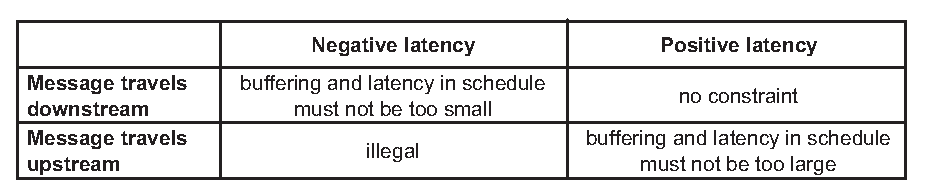
\psfig{file=constraints.eps,width=3in}
\vspace{-4pt}
\caption{\small Scheduling constraints imposed by messages.}
%% {\small
%% \begin{tabular}{|r|c|c|} \hline
%% ~ & {\bf Negative latency} & {\bf Positive latency} \\ \hline
%% {\bf Message travels downstream} & buffering and latency in schedule must not be too small & no constraint \\ \hline
%% {\bf Message travels upstream} & illegal & buffering and latency in schedule must not be too big \\ \hline
%% \end{tabular}}
\label{tab:messcons}
\end{center}
\vspace{-18pt}
\end{figure}

For upstream messages with negative latency, there always exist
iterations of the sender during which any messages sent are
impossible to deliver.  Consider an iteration of the sender that is
the first to depend on data propagating from the $n$th execution of
the receiver.  A negative-latency message would be delivered
immediately after a {\it previous} iteration of the receiver, but
since iteration $n$ has already fired, the message is impossible to
deliver.  Conversely, a downstream message with positive or zero
latency imposes no constraint on the schedule, as the sender has not
yet produced the data that is synchronized with the message.

\paragraph*{Unsatisfiable Constraints}  
Messaging constraints can be unsatisfiable---that is, assuming a
message is sent on every iteration of the sender's work function,
there does not exist a schedule that delivers all of the messages
within the desired latency range.  Such constraints should result in a
compile-time error.  

Figure~\ref{fig:infeasible} illustrates an example of unsatisfiable
constraints.  Though each messaging constraint is feasible in
isolation, the set of constraints together is unsatisfiable.  The
unsatisfiability is caused by conflicting demands on the buffering
between B and C.  The message from B to C constrains this buffer to
contain at least 10 items, while the message from D to A constrains it
to be empty.  We say that these two constraints {\it overlap} because
the paths from sender to receiver intersect a common actor in the
stream graph.
\begin{figure}[t]
\begin{center}
\psfig{figure=infeasible-messaging.eps,height=1.43in}
\vspace{-8pt}
\caption{{\small Example of unsatisfiable message constraints.  Each
node is annotated with its input and output rate.  Messages are shown
by dotted arrows, drawn from sender to receiver with a given latency.
The constraints are satisfiable in isolation, but unsatisfiable in
combination.  \protect\label{fig:infeasible}}}
\end{center}
\vspace{-13pt}
\end{figure}

\paragraph*{Finding a Schedule}
In the presence of overlapping constraints, we leave to future work
the problem of finding a legal execution schedule (if one exists).
Because overlapping constraints can be detected statically, a given
compiler may choose to prohibit overlapping constraints altogether.
%A discussion of the issues involved appears in a
%thesis~\cite{karczma-thesis} by one of the authors.

\begin{figure}[t]
\vspace{-12pt}
\centering
\psfig{figure=fhr-streamit.eps,width=2.841in}
\vspace{-8pt}
\caption{\small Stream graph of frequency hopping radio with teleport messaging.  
A portal delivers point-to-point latency-constrained messages from the
detectors to the RFtoIF stage.
\protect\label{fig:fhr-streamit}}
\vspace{-12pt}
\end{figure}

\begin{figure}[t]
\vspace{-12pt}
\hspace{-0.2in}\psfig{figure=code-freq1.eps,width=3.5in}
\vspace{-24pt}
\caption{\small Frequency hopping radio with teleport messaging.
Arrows depict the path of messages from the sender to the receiver,
via a portal declared in the top-level stream.
\protect\label{fig:freq1}}
\vspace{-12pt}
\end{figure}


For the case of non-overlapping constraints, a simple modification to
pull scheduling will always result in a legal schedule (if one
exists).  First, note that a pull schedule always satisfies
constraints imposed by upstream messages; because upstream (receiving)
actors execute as little as possible per execution of the downstream
(sending) actor, a message can be forwarded to the receiver
immediately after sending.  The receiver can then store the message
and process it at the appropriate iteration.  For downstream messages,
the pull scheduler is modified to always execute one iteration of the
upstream (sending) actor before any execution of the downstream
(receiving) actor that would exceed the latency range.  If the
upstream actor needs more inputs to fire, then they can always be
generated by actors that are further upstream (via a recursive call to
the pull scheduling algorithm).

As described in Section~\ref{sec:evaluation}, our compiler uses a
simple implementation of messaging in which each sender or receiver
executes in its own thread and waits for possible messages at
appropriate iterations.  This approach does not depend on producing a
serial ordering of the actors at compile time.

%\begin{figure}[t]
\begin{center}
\psfig{figure=constrained-example.eps,height=1.5in}
\caption{{\small Example of construction of a constrained schedule. The $\sdepf{R}{S}$ function for filters $R$ and $S$ is given in Table \ref{tab:sdepconst}. The blob between filters $R$ and $S$ illustrates other possible stream elements. $R$ sends a message to $S$ with latency $[1,2]$. Executions of the blob are omitted, it is assumed that at the point $S$ executes, the blob has drained data provided by $R$.}}
\end{center}
\vspace{-12pt}
\label{fig:sdepconst}
\end{figure}

\begin{table*}[t]
{\small
\begin{tabular}{|c|c|} \hline
{\bf $sdepf{R}{S}$} & {\bf Execs of S} \\ \hline
$9n+2$ & $8n+1$ \\ \hline
$9n+3$ & $8n+2$ \\ \hline
$9n+5$ & $8n+3$ \\ \hline
$9n+5$ & $8n+4$ \\ \hline
$9n+6$ & $8n+5$ \\ \hline
$9n+8$ & $8n+6$ \\ \hline
$9n+9$ & $8n+7$ \\ \hline
$9n+9$ & $8n+8$ \\ \hline
\end{tabular}}
\caption{\small $sdepf{R}{S}$ function for example in Figure \ref{fig:sdepconst}. This particular $\sdep$ function was obtained by setting $push_R=2$, $pop_S=3$ and making the blob between $R$ and $S$ into a filter that pops 3 and pushes 4 every iteration of its work function. No initialization due to peeking is necessary in this example.}
\label{tab:sdepconst}
\end{table*}


Explanation of working of the example:

The example in Figure \ref{fig:sdepconst} illustrates scheduling of a single constraint. The constraint is a message sent upstream with latency $[1,2]$. The resulting schedule consists of two parts, an initialization schedule and a steady state schedule. The initialization schedule is necessary to initialize the constraint, to ensure that the steady schedule can be executed repeatedly forever. Notation used here is: $lastReceived$ denotes the execution of S which sent the last message to be received by R; $n_S$ indicates number of executions of $S$ and $n_R$ indicates number of executions of $R$.

Initialization schedule is computed by executing R $SDEP(minLatency)-1$ number of times, and executing S as many times as possible, given data provided by R. This assures that when the steady schedule starts, all executions of filters will contribute to new message sending and receiving, thus allowing the steady state schedule to execute forever. The initialization schedule does not need to send or receive messages here.

The steady state schedule is computed by executing the receiver R as far as possible without going beyond the boundary of being able to receive message sent by S on execution $lastReceived+1$ (indicated by "Oldest msg to receive" in the figure). Now the sender S is executed as many times as possible, given data provided by R. Now S can receive messages sent by S in its executions $[lastReceived+1 ... \min(n_S, $"Newest msg to receive"$)]$.

"Oldest msg to receive" is equal to $iSDEP(n_R)-maxLatency$. "Newest msg to receive" is equal to $m-minLatency$ with $m$ being the greatest integer such that $SDEP(m) \le n_R$.


\section{Case Study}
\label{sec:casestudy}

To illustrate the pros and cons of teleport messaging, we implemented
a spread-spectrum frequency hopping radio frontend~\cite{harada02} as
shown in Figure~\ref{fig:fhr-streamit}.  A frequency hopping radio is
one in which the receiver switches between a set of known frequencies
whenever it detects certain tones from the transmitter.  The frequency
hopping is a good match for control messages because the hopping
interval is dynamic (based on data in the stream); it spans a large
section of the stream graph (there is a Fast Fourier Transform (FFT)
with 15 child actors, not shown, between the demodulator and the hop
detector); and it requires precise message delivery.  The delivery
must be precise both to meet real-time requirements (as the
transmitter will leave the current frequency soon), and to ensure that
the message falls at a logical frame boundary; if the frequency change
is out of sync with the FFT, then the FFT will muddle the spectrum of
the old and new frequency bands.

A StreamIt version of the radio frontend with teleport messaging
appears in Figure~\ref{fig:freq1}.  The FreqHoppingRadio pipeline
creates a portal and adds the RFtoIF actor as a receiver (lines 45 and
48 respectively).  The portal is passed to the CheckFreqHop stage,
where four parallel detectors send messages into the portal if they
detect a hop in the frequency they are monitoring (lines 32-35).  The
messages are sent with a latency of 6 to ensure a timely transition.
To make sense of the latency, note that $\sdepf{RFtoIF}{D}(n) = 512*n$
for each of the detector actors $D$.  This comes about because the FFT
stage consumes and produces 512 items\footnote{\small Though the FFT is
256-way, the real and imaginary parts are interleaved on the tape,
leading to an I/O rate of 512.}; each detector fires once per set of
outputs from the FFT, but RFtoIF fires 512 times to fill the FFT
input.  Because of this $\sdep$ relationship, messages sent from the
detectors to RFtoIF are guaranteed to arrive only at iterations that
are a multiple of 512.  This satisfies the design criterion that a
given FFT stage will not operate on data that were demodulated at two
separate frequencies.

\begin{figure}[t]
\centering
\psfig{figure=fhr-feedback.eps,width=3.13in}
\caption{\small Stream graph of frequency hopping radio with control
messages implemented manually.  A feedback loop connects the detectors
with the RFtoIF stage, and an item is sent on every invocation to
indicate whether or not a message is present.  The latency and
periodicity of message delivery are governed by the data rates and the
number of items on the feedback
path. \protect\label{fig:fhr-manual}}
\end{figure}

Another version of the frequency hopping radio appears in
Figures~\ref{fig:fhr-manual} and~\ref{fig:freq2}.  This version is
functionally equivalent to the first, except that the control messages
are implemented manually by embedding them in the data stream and
in-
%
\begin{figure}[t]
\vspace{-26pt}
\hspace{-0.2in}\psfig{figure=code-freq2.eps,width=3.5in}
\vspace{-20pt}
\caption{\small Frequency hopping radio with manual feedback loop for
event handling.  Lines that differ from Figure~\ref{fig:freq1} are
marked with an asterisk. \protect\label{fig:freq2}}
\vspace{-12pt}
\end{figure}

\clearpage
\noindent
troducing a feedback loop.  Because the number of items transfered
around the loop must be constant from one iteration to the next, a
data item is sent whether or not there is a message as part of the
algorithm.  The RFtoIF filter checks the values from the loop on every
iteration; if the value is non-zero, it is treated as a message (the
new frequency), while a value of zero is ignored (no message).  The
I/O rate of the RFtoIF filter has been scaled up to ensure that the
messaging information is received at intervals of 512 iterations (as
in the version with portals).  To achieve the desired messaging
latency of 6 frames, $6*256 = 1536$ items are enqueued on the feedback
path prior to execution.

%% As described previously, yet another way to approximate the behavior
%% of messaging is with a direct function call from the detector to the
%% RFtoIF stage.  (Though such a call is disallowed in StreamIt, it could
%% be an option in a different programming model.)  While this approach
%% is simple, it does not have any timing guarantees.  Because the sender
%% and receiver are running in parallel, there is no way for the sender
%% to know when in the course of the receiver's execution the message
%% will be received.  This could cause problems both for algorithm
%% development and for the reliability and predictability of software.

\subsection{Discussion}

Teleport messaging offers several benefits compared to a manual
implementation of equivalent functionality.  While embedding messages
in the data stream is equally precise, it involves several tedious
and error-prone changes, not only to the stream graph but also to the
steady-state execution code within the actors.  In particular, the
manual derivation of the loop delay, adjustment of the actor I/O
rates, and implicit interleaving of data items with control messages
has a negative impact on the readability and maintainability of the
code.  Teleport messaging provides the same level of precision, but
with the simplicity of a method call.

Teleport messaging also has advantages from a compiler standpoint.  By
separating the data-intensive code from the control-oriented code, the
common case of steady-state execution is not sacrificed for
the uncommon case of message processing.  There are no ``dummy items''
serving as placeholders in the static-rate channels.  In addition, by
exposing the message latency as part of the language, the compiler can
infer the true dependences between actor firings and reorder the
execution so long as the message constraints are respected.  The
actual message delivery can be implemented in the most efficient way
for a given architecture.

A final benefit of teleport messaging is the clean interface provided
by the portals.  Since a portal can have multiple receivers, it is
straightforward to send a message that is delivered synchronously to
two actors in parallel streams.  For example, consider a vocoder (an
encoder for voice signals) that is separately manipulating the
magnitude and phase components of a signal.  If something triggers an
adjustment to the speech transformation (e.g., the speaker
requests a change of pitch) then the mask needs to be updated at the
same time relative to data in both parallel streams.  A portal that
contains both components seamlessly provides this functionality.
Finally, portals are useful as an external programming interface; an
application can export a portal based on an interface type without
exposing the underlying actor implementation.

One aspect of teleport messaging might be considered unusual: the
granularity of message delivery can be affected by changes in
granularity elsewhere in the stream graph.  This is evident in the
frequency hopping radio, as the I/O rate of 512 on the FFT implies
that the RFToIF stage will receive messages from CheckFreqHop at most
once every 512 iterations.  (If the FFT were coarsened to 1024-way,
the granularity of messages in RFToIF would increase accordingly.)  In
this case the behavior is desirable, as messages should not interrupt
frame boundaries.  It seems that in many cases, the I/O rates are
meaningful aspects of the program and their influence on message
granularity is appropriate.  Nonetheless, this non-local influence
might come as a surprise to programmers.  If the FFT granularity is
scaled up for a different reason (e.g., caching behavior), the effects
on message granularity might be unwanted.

This suggests that it might be worthwhile, in future work, to
investigate additional mechanisms for programmers to specify the
messaging contract independently of the declared I/O rates.  For
example, a parent stream could override the I/O rates of a child for
the sake of a given $\sdep$ calculation.  The scheduler would deliver
messages according to the parent's expectation of $\sdep$, or report
an error if such delivery is incompatible with the actual I/O rates.

\newpage

\section{Dynamic Morphing}
\label{sec:morphing}

\section{Future Additions}

This section describes features that are likely to be present in a
future release of the language.

\subsection{The \lstinline|keep| Construct}

The \lstinline|keep| function will look at, but not remove, items on
the output tape of a filter.  \lstinline|keep(0)| returns the item
that was most recently pushed, even if that was on a previous filter
iteration.  Just as \lstinline|pop| affects indices for future
\lstinline|peek| calls, \lstinline|push| adds another item to the
output tape and hence changes the indices for future \lstinline|keep|
calls.

\lstinline|keep| can be used to implement IIR filters.  For example,
given this LTI filter:

\begin{eqnarray*}
H(z) & = & \frac{1+z^{-1}}{1-z^{-1}} \\
(1-z^{-1}) Y(z) & = & (1+z^{-1}) X(z) \\
y[n] - y[n-1] & = & x[n] + x[n-1] \\
y[n] & = & x[n] + x[n-1] + y[n-1] \\
\end{eqnarray*}

We can write equivalent StreamIt code:

\begin{lstlisting}{}
float->float filter IIRExample {
  prework push 1 {
    push(0);
  }
  work push 1 pop 1 peek 2 keep 1 {
    // y[n] = x[n] + x[n-1] + y[n-1]
    push(peek(0) + peek(1) + keep(0));
    pop();
  }
}
\end{lstlisting}

Of note, since the work function can not fire unless there is at least
one item on its output tape, there must be a prework function that
pushes that item; otherwise, the program is unschedulable.

\subsection{Helper Packages}

In many cases the programmer would benefit from writing a set of
stateless helper functions that can be used in multiple filters.  For
example, the GSM encoder we have now uses the C preprocessor to
include a set of functions to perform 16-bit arithmetic.  Syntax for
this functionality does not yet exist, though we may create a
\lstinline|static| keyword:

\begin{lstlisting}{}
static MyHelpers {
  int square(int x) { return x * x; }
}
int->int filter SquareIt {
  work pop 1 push 1 { push(MyHelpers.square(pop())); }
}
\end{lstlisting}

%\section{Future Changes}

This section describes features that may appear in future versions of
StreamIt.

\subsection{Additional Primitive Types}

Support for characters and strings is somewhat uncertain.  There is no
particular use for a character primitive type in StreamIt at the
moment, though a byte type may be useful for reading in files.
Strings may be useful for debugging code, and for file name parameters
to file reader and writer objects.

\subsection{Parameterized Types}

StreamIt should allow parameterized types, using a syntax similar to
C++'s \lstinline|template| construct.  For example, one might write:

\begin{lstlisting}{}
template<T> T->T filter Duplicate {
  work pop 1 push 2 {
    T val = pop();
    push(val);
    push(val);
  }
}
\end{lstlisting}

Then \lstinline|Duplicate<int>| would be a stream type that duplicates
integers.

There is some disagreement on how to implement array types.  The
language currently accepts \lstinline|int[N]->int[N] filter Name(int N)| to
have a specified-length array.  It may be better to use a template
construct for this, though then value parameters can appear in two
different places in the code.

\subsection{Messaging Extensions}

Future versions of StreamIt may have two extensions to the existing
messaging system.  First, an \emph{interface}, much like a Java
interface, may be declared, and filters may declare that they
implement an interface.  Then a portal to an interface type may be
declared, and filters of any implementing type may be added.  Second,
we may lift the restriction that only filters may receive messages.

\subsection{Reinitialization}

We might occasionally want to change parts of the stream graph at
runtime, or to change the static parameters of the program.  This is a
major effort the way StreamIt code is currently constructed.  The CC
paper proposed sending an \lstinline|init| message through a portal to
perform reinitialization; this would result in the targets'
\lstinline|init| functions being re-run.

This is simple enough for filters, though some state in the filter may
be lost that reinitialization would want to be preserved.  What
happens for composite streams, though?  Are their children destroyed
and reborn, or are individual children added and removed?  What syntax
is necessary for this?

\subsection{Variable Rates}

Certain types of applications, such as those involving compression
algorithms, do not have a fixed ratio of outputs to inputs.  StreamIt
does not currently support variable rates.  The current proposal is
that variable rates will be accomodated by phased filters: one phase
reads the input, and then runs another phase for a certain number of
executions that writes the output, with the number of executions being
variable.

It is still possible that dedicated syntax for variable rates will be
added.  This will likely accomodate bounds on the I/O rates of the
filter, since a filter might read four bytes of input and produce
between two and sixteen bytes of output; having this information can
assist the scheduler.

\subsection{Static Control Flow and Dynamic Phases}

This document should contain a discussion of the notion of
\emph{static control flow}.  This is essentially a requirement that
the path through a given control flow graph is determinable at compile
time; loops can be fully unrolled, and every branch can be
determined.  This extends the concept of compile-time constancy
already covered.

This would allow us to refine the current description of phases.  In
particular, we want the current phase specification to be entirely
specified by static control.  As a future extension, the control flow
can be dynamic, to allow data-dependent phase execution.  This can be
used to implement some forms of dynamic-rate filters.  For example:

\begin{lstlisting}{}
// Format: #reps, #bytes, data
byte->byte filter RLEExpand {
  byte data[256];
  int reps, count;
  work {
    readReps();
    readCount();
    for (int i = 0; i < count; i++)
      readData(i);
    for (int i = 0; i < reps; i++)
      writeData(count);
  }
  phase readReps pop 1 { reps = pop(); }
  phase readCount pop 1 { count = pop(); }
  phase readData(int pos) pop 1 { data[pos] = pop(); }
  phase writeData() push count {
    for (int i = 0; i < count; i++)
      push(data[i]);
  }
}
\end{lstlisting}

Note that the number of executions of the \lstinline|readData| and
\lstinline|writeData| phases are data-dependent, as is the
\lstinline|push| rate of \lstinline|writeData|.

%% \section{Implementation Limits}

%% The following limits apply to the current implementation of StreamIt:

%% \begin{itemize}
%% \item There is no guaranteed order of evaluation.  In particular, a
%%   statement in a work function should not contain more than a single
%%   \lstinline|pop()|, and if contains any \lstinline|pop()|s at all, it
%%   should contain no \lstinline|peek()|s.
  
%% \item The names \lstinline|SplitJoin|, \lstinline|FeedbackLoop|,
%%   \lstinline|Filter|, \lstinline|Pipeline|, \lstinline|StreamIt|, and
%%   \lstinline|Complex| are reserved.  Certain variable names beginning
%%   with underscores may cause conflicts if used as local variables.

%% \end{itemize}

\section{History}

\subsection{StreamIt 2.0}

The first formal language specification for StreamIt documented
StreamIt 2.0.  Version 2.0 of the language adds a completely new
syntax with simplified constructs for declaring stream objects but
keeping a Java-like syntax for the bodies of init and work functions.
It also changes
%Other new features include \lstinline|prework| functions, phased
%filters, messaging, the \lstinline|keep| expression, and changing 
from delay functions to \lstinline|enqueue| statements in feedback
loops.  The \lstinline|null| splitter/joiner type was replaced with
\lstinline|roundrobin(0)|.

\subsection{StreamIt 1.0}

The initial StreamIt compiler was based on a restricted subset of
Java, dubbed StreamIt 1.0.  This version of the language used pure
Java syntax for stream constructs, and was compilable with a normal
Java compiler given an appropriate run-time library.  Early
publications referred to the language as StreaMIT, but this
capitalization is now deprecated.

\bibliographystyle{abbrv}
\bibliography{references}

\end{document}